%!TeX program = xelatex
% VizDOM - Tài liệu Kiến trúc arc42 (Tiếng Việt). Biên dịch bằng XeLaTeX (xem README.md).
% Overleaf: Menu -> Settings -> Compiler -> XeLaTeX (fontspec cần XeTeX/LuaTeX).
\documentclass[11pt,a4paper]{report}

\usepackage{fontspec}
\usepackage[vietnamese]{babel}
\usepackage{microtype}
\usepackage{geometry}
\geometry{margin=2.4cm}
\usepackage{graphicx}
\usepackage{booktabs}
\usepackage{array}
\usepackage{longtable}
\usepackage{caption}
\usepackage{enumitem}
\usepackage{xcolor}
\usepackage[hidelinks]{hyperref}
\usepackage{float}
\usepackage{titlesec}

\graphicspath{{figures/}}
\newcommand{\code}[1]{\texttt{#1}}
\newcommand{\req}[1]{\textbf{#1}}
\setlength{\parskip}{0.4em}
\setlength{\parindent}{0pt}
\setlength{\tabcolsep}{4pt}
\renewcommand{\arraystretch}{1.25}

\titleformat{\chapter}[hang]{\normalfont\huge\bfseries}{\thechapter}{1em}{}
\titlespacing*{\chapter}{0pt}{0pt}{1em}

\title{\textbf{VizDOM --- Tài liệu Kiến trúc}\\[0.3em]
\large Theo khuôn mẫu arc42}
\author{Nguyễn Huỳnh Trí Cương\\
\small Đồ án ứng dụng thạc sĩ (Ngành Khoa học máy tính) --- Đại học Khoa học Tự nhiên TP. Hồ Chí Minh\\
\small Khoa Công nghệ thông tin\\
\small Giảng viên hướng dẫn: PGS.TS Nguyễn Văn Vũ}
\date{2026 --- Bản 1.0}

\begin{document}
\maketitle

\begin{abstract}
\noindent Tài liệu này mô tả kiến trúc phần mềm của \textbf{VizDOM}, một hệ thống tái
dựng cây DOM (Document Object Model) tương tự UI Automator từ một ảnh chụp màn hình
GUI, nhằm cho phép kiểm thử tự động các ứng dụng không cung cấp cây trợ năng. Tài
liệu tuân theo khuôn mẫu arc42 và kỷ luật quyết định SWA
(drivers~$\rightarrow$~giải pháp~$\rightarrow$~tài liệu~$\rightarrow$~kiểm chứng).
Nguyên tắc chủ đạo là khả truy vết: mọi lựa chọn có ý nghĩa kiến trúc đều gắn với một
driver được xếp hạng và, khi có thể, với bằng chứng đo được. VizDOM là một đồ án ứng
dụng theo Phương thức 3; kiến trúc nhấn mạnh khả sửa đổi (bộ phát hiện/chụp/tác động
cắm-thay được), khả triển khai (mỗi mối quan tâm chạy được tại chỗ hoặc như một dịch
vụ gRPC từ xa) và khả kiểm thử, hơn là tính mới của thuật toán.
\end{abstract}

\tableofcontents

% =====================================================================
\chapter{Giới thiệu và Mục tiêu}
% =====================================================================
VizDOM chuyển một \emph{ảnh chụp màn hình} GUI thành một \emph{Visual DOM} có cấu trúc,
truy vấn được --- khung bao phần tử, vai trò, văn bản, nhãn, bộ định vị và phân cấp
--- bằng thị giác máy tính cộng một mô hình ngôn ngữ/thị giác nhỏ, rồi cung cấp DOM đó
cho một khung kiểm thử. Nó nhắm tới các ứng dụng nơi cây trợ năng nền tảng (Android
UI~Automator, Windows~UIA, DOM của web) vắng mặt hoặc không đáng tin: giao diện
desktop vẽ tùy biến (Qt/QML, OpenGL, game engine), HMI nhúng/công nghiệp, và màn hình
quan sát qua camera. Nơi có cây trợ năng, các khung như Appium dựa vào
nó~\cite{uiautomator,appium}; VizDOM nhắm tới các trường hợp không có.

\paragraph{Bối cảnh vấn đề.} Phát hiện phần tử GUI khó hơn phát hiện đối tượng trong
ảnh tự nhiên: ở cấp phần tử, một lớp biến thiên lớn (biến thiên trong cùng lớp) trong
khi các lớp khác nhau trông giống nhau (tương đồng giữa các lớp); ở cấp GUI, widget,
hình ảnh và văn bản trộn lẫn, các phần tử xếp dày đặc, và kiểm thử cần hộp độ chính
xác cao chứ không phải một vùng lỏng lẻo~\cite{xie2020uied}. Không họ bộ phát hiện nào
--- cổ điển hay học sâu --- trội đều trên các điều kiện này. Đây là động lực kiến trúc
đứng sau quyết định bộ phát hiện cắm-thay được (ADR-015) và các bước làm sạch; báo cáo
dự án trình bày đầy đủ phạm vi vấn đề/giải pháp.

\section{Tổng quan yêu cầu}
\subsection*{Yêu cầu chức năng}
\begin{longtable}{@{}p{1.6cm}p{12.6cm}@{}}
\toprule
\textbf{ID} & \textbf{Yêu cầu chức năng} \\
\midrule
\endhead
FR1 & Thu nhận ảnh chụp từ một nguồn cấu hình được (desktop OS, thiết bị Android, camera, dịch vụ từ xa, hoặc tệp). \\
FR2 & Phát hiện phần tử UI và văn bản trong ảnh bằng một backend phát hiện chọn được. \\
FR3 & Ghép các phát hiện thành phân cấp và biên dịch một DOM tương tự UI Automator (vai trò, cờ, nhãn, nhiều bộ định vị). \\
FR4 & Phân giải một bộ định vị (theo id/text/hint/role/quan hệ không gian) thành một phần tử cụ thể. \\
FR5 & Điều khiển đầu vào (bấm, gõ, phím, cuộn, kéo) trên một phần tử đã phân giải. \\
FR6 & Cung cấp các chức năng trên cho Robot Framework dưới dạng từ khóa. \\
FR7 & Cho phép chụp, phát hiện và tác động chạy như các dịch vụ từ xa trên nhiều máy/thiết bị. \\
FR8 & Cho phép người dùng thêm backend phát hiện/chụp/tác động mới mà không sửa lõi. \\
\bottomrule
\end{longtable}

\subsection*{Yêu cầu chất lượng (đo được)}
\begin{longtable}{@{}p{1.6cm}p{4.0cm}p{8.6cm}@{}}
\toprule
\textbf{ID} & \textbf{Chất lượng} & \textbf{Phát biểu đo được} \\
\midrule
\endhead
NFR1 & Khả sửa đổi & Thêm một backend phát hiện/chụp/tác động mới bằng cách thêm một tệp và một mục registry, với \textbf{không} sửa đổi lõi nghiệp vụ; mỗi cổng có $\geq 2$ hiện thực hoán đổi được. \\
NFR2 & Khả triển khai & Mỗi cổng chọn được là \emph{tại chỗ} hay \emph{gRPC} thuần bằng cấu hình; luồng chụp$\rightarrow$phát hiện$\rightarrow$tác động chạy không đổi trên $\geq 2$ máy. \\
NFR3 & Hiệu năng & Một dịch vụ phát hiện nạp mô hình \textbf{một lần} (mô hình nóng) và phục vụ các yêu cầu sau mà không nạp lại; độ trễ mỗi yêu cầu không tính thời gian nạp mô hình. \\
NFR4 & Khả kiểm thử & Lõi nghiệp vụ chạy đầu-cuối không cần GPU và không cần mạng (bộ phát hiện UIED + chụp static-image + bộ tác động ghi lại). \\
NFR5 & Độ chính xác & Mục tiêu: phát hiện phần tử F1 $\geq 0.80$ và IoU trung bình $\geq 0.60$ trên điểm chuẩn gán nhãn. Đo được (tập tổng hợp 44 ảnh): F1 tổng thể $0.58$ (OmniParser) / $0.51$ (UIED), mIoU 0.67--0.68 --- đạt mục tiêu mIoU, \emph{chưa} đạt mục tiêu F1. Theo loại, OmniParser trội trên các điều khiển thao tác được (nút 1.00, input\_field 0.99, biểu tượng 0.67) còn UIED trên hộp kiểm/văn bản; cả hai đều bấm-trúng-được (center-hit: OmniParser thao tác được 0.97, UIED 0.89). Xem Ch.~10--11. \\
\bottomrule
\end{longtable}

\section{Mục tiêu chất lượng (3 hàng đầu)}
\begin{enumerate}[leftmargin=1.6em]
  \item \req{Khả sửa đổi / mở rộng} --- hoán đổi và thêm backend là ý định thiết kế
        trung tâm; giá trị của hệ thống nằm ở chỗ các bộ phát hiện cổ điển và học máy,
        cùng các thiết bị chụp/tác động đa dạng, đều hoán đổi được.
  \item \req{Khả triển khai} --- chụp chạy nơi ứng dụng cần kiểm thử, phát hiện hưởng
        lợi từ GPU, tác động xảy ra tại thiết bị hoặc bộ điều khiển vật lý; kiến trúc
        phải cho phép các phần này nằm trên các máy khác nhau.
  \item \req{Khả kiểm thử} --- pipeline và tầng Robot Framework phải kiểm chứng được
        mà không cần phần cứng đặc biệt, để dự án phát triển và chấm điểm được trên
        một laptop.
\end{enumerate}

\section{Các bên liên quan}
\begin{longtable}{@{}p{3.4cm}p{2.2cm}p{2.0cm}p{6.0cm}@{}}
\toprule
\textbf{Bên liên quan} & \textbf{Quan tâm} & \textbf{Quyền lực} & \textbf{Nhu cầu chính} \\
\midrule
\endhead
Học viên / tác giả & Cao & Cao & Một hệ thống ứng dụng và báo cáo hoạt động được, bảo vệ được. \\
GVHD / hội đồng & Cao & Cao & Kỹ thuật rõ ràng, quyết định truy vết được, đánh giá trung thực. \\
Kỹ sư kiểm thử (người dùng) & Cao & Thấp & Định vị phần tử tin cậy trên UI không trợ năng; từ khóa đơn giản. \\
Kỹ sư tích hợp thiết bị/robot & Trung bình & Thấp & Một điểm cắm để gắn camera / cánh tay robot. \\
Vận hành (tương lai) & Thấp & Thấp & Dịch vụ khởi động, ghi log và lỗi an toàn. \\
\bottomrule
\end{longtable}

% =====================================================================
\chapter{Ràng buộc Kiến trúc}
% =====================================================================
\begin{longtable}{@{}p{3.6cm}p{11.0cm}@{}}
\toprule
\textbf{Ràng buộc} & \textbf{Chi tiết và hệ quả} \\
\midrule
\endhead
Môi trường chạy & Python 3.9 với bản dựng PyTorch hỗ trợ CUDA (cu124); trình thông dịch đang dùng không được bị công cụ môi trường làm xáo trộn. \\
Quản lý môi trường & Dùng \code{uv} trên trình thông dịch sẵn có (không tái tạo bản dựng CUDA đang chạy). \\
Proxy doanh nghiệp & Các kho mã công khai (GitHub, Maven) bị chặn; PyPI và chỉ mục PyTorch truy cập được. Mã mô hình ngoài được \emph{đóng gói kèm và ghim} bằng script cài đặt, không phải submodule; tài liệu kết xuất UML \emph{ngoại tuyến} từ bộ kết xuất cục bộ. \\
Không dùng container & Docker/Nomad/Consul bị loại trừ rõ ràng (tốn tài nguyên); phân tán dùng tiến trình gRPC thuần và script khởi chạy. \\
Ghim phụ thuộc & \code{protobuf < 6} toàn dự án (xung đột Streamlit/TensorFlow); \code{grpcio}/\code{grpcio-tools} ghim tương ứng. \\
Giấy phép & Bộ phát hiện biểu tượng của OmniParser là AGPL-3.0 (qua Ultralytics); phục vụ backend đó qua mạng kèm nghĩa vụ AGPL. UIED vẫn là đường cơ sở CPU không dính AGPL. \\
Sơ đồ & Mã nguồn PlantUML chỉ dùng ASCII và kết xuất qua jar đóng gói kèm (bố cục Smetana; \code{architecture.puml} dùng Graphviz). \\
Loại dự án & Đồ án ứng dụng Phương thức 3: kỹ thuật vững có nội dung khoa học, không phải luận văn thuật toán mới. \\
\bottomrule
\end{longtable}

% =====================================================================
\chapter{Bối cảnh và Phạm vi}
% =====================================================================
\section{Bối cảnh nghiệp vụ}
VizDOM nằm giữa một \emph{màn hình} (ứng dụng cần kiểm thử) và một \emph{khung kiểm
thử}. Giao diện vào là một ảnh; giao diện ra là một DOM cộng khả năng tác động đầu
vào. Hình~\ref{fig:overview} minh họa luồng đầu-cuối.

\begin{figure}[H]
  \centering
  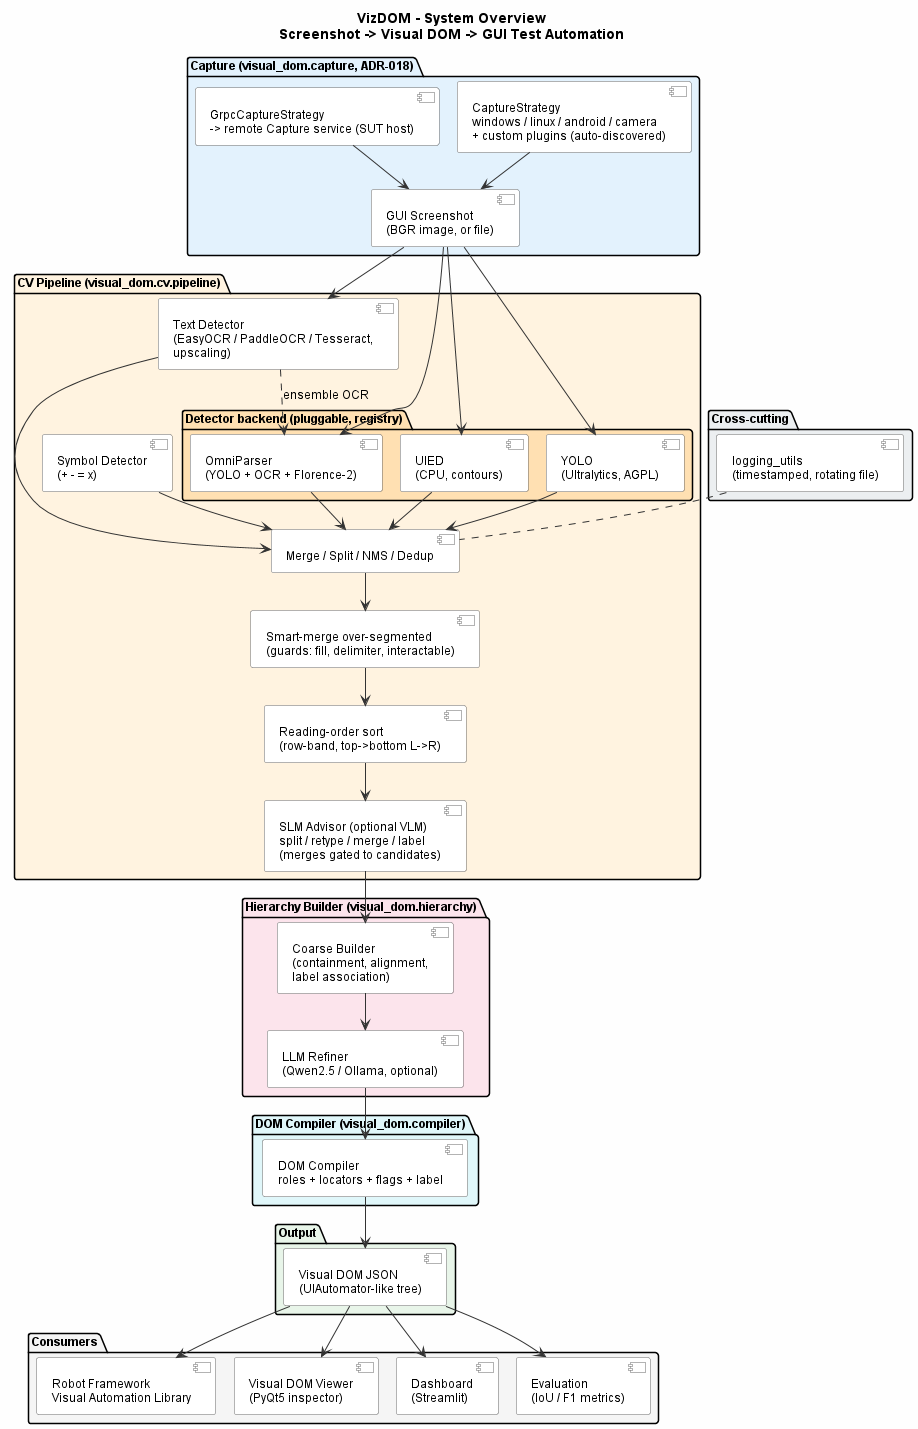
\includegraphics[width=0.6\linewidth]{System_Overview.png}
  \caption{Tổng quan / bối cảnh hệ thống. Ranh giới trái: một ảnh chụp từ bất kỳ
  nguồn chụp nào. Ranh giới phải: một Visual DOM được tiêu thụ bởi Robot Framework,
  trình xem, bảng điều khiển và bộ khung đánh giá. Chú giải: gói tô màu là hệ thống
  con; mũi tên là luồng dữ liệu/điều khiển.}
  \label{fig:overview}
\end{figure}

\section{Bối cảnh kỹ thuật (giao diện)}
\begin{longtable}{@{}p{3.4cm}p{3.0cm}p{7.6cm}@{}}
\toprule
\textbf{Lân cận} & \textbf{Hướng} & \textbf{Giao diện} \\
\midrule
\endhead
Ứng dụng cần kiểm thử & vào & Ảnh chụp (BGR) qua một chiến lược chụp; sự kiện đầu vào qua một chiến lược tác động. \\
Bộ OCR & ra & EasyOCR~\cite{easyocr} / PaddleOCR / Tesseract~\cite{tesseract} (thư viện trong tiến trình). \\
OmniParser & ra & Repo đóng gói kèm~\cite{omniparser2024} + trọng số Florence-2~\cite{florence2} / YOLO~\cite{ultralytics} (tệp cục bộ). \\
Ollama & ra & HTTP tới một LM/VLM nhỏ cục bộ/từ xa cho tinh chỉnh tùy chọn. \\
Dịch vụ từ xa & cả hai & gRPC~\cite{grpc}: phát hiện (\code{:50051}), chụp (\code{:50053}), tác động (\code{:50054}). \\
Robot Framework & vào & Thư viện từ khóa (Python)~\cite{robotframework} tiêu thụ DOM. \\
\bottomrule
\end{longtable}

\section{Phạm vi}
\textbf{Trong phạm vi:} thu nhận ảnh, phát hiện phần tử/văn bản, tổng hợp DOM, phân
giải bộ định vị, tác động đầu vào, thư viện Robot Framework, và lớp truyền dịch vụ
phân tán. \textbf{Ngoài phạm vi:} soạn và lập lịch ca kiểm thử (để cho Robot
Framework), một dịch vụ đa người thuê được host, xác thực các kênh gRPC (ghi nhận là
nợ kỹ thuật), và mọi thay đổi tới ứng dụng cần kiểm thử.

% =====================================================================
\chapter{Chiến lược Giải pháp}
% =====================================================================
\section{Tóm tắt chiến lược}
\begin{longtable}{@{}p{3.4cm}p{11.2cm}@{}}
\toprule
\textbf{Mục tiêu chất lượng} & \textbf{Cách tiếp cận kiến trúc} \\
\midrule
\endhead
Khả sửa đổi & \emph{Lục giác (ports \& adapters)}: một lõi nghiệp vụ thuần chỉ phụ thuộc các cổng trừu tượng (Detector, Ocr, Refiner, Capture, Actuator). Mỗi cổng dùng khuôn mẫu \emph{strategy + registry + tự khám phá}, nên backend được thêm dưới dạng plugin. \\
Khả triển khai & Mỗi cổng bị điều khiển có một bộ điều hợp tại chỗ \emph{và} một bộ điều hợp gRPC-client; một máy chủ gRPC tương ứng bọc registry trên máy từ xa. Truyền tải là lựa chọn cấu hình theo cổng, không phải viết lại. \\
Hiệu năng & Dịch vụ mô hình là \emph{nóng}: nạp một mô hình nặng một lần và phục vụ nhiều client nhẹ, khấu hao chi phí nạp. \\
Khả kiểm thử & Lõi không có I/O và phụ thuộc các cổng; một bộ phát hiện CPU không phụ thuộc thư viện (UIED), một chụp static-image, và một bộ tác động ghi lại giúp chạy đầy đủ mà không cần GPU và mạng. \\
Độ chính xác & Một bộ phát hiện học máy cắm-thay được (OmniParser) cộng tổng hợp OCR và một bước tinh chỉnh có kiểm soát bằng mô hình nhỏ; UIED cổ điển làm đường cơ sở. \\
\bottomrule
\end{longtable}

\section{Xếp hạng driver}
Bối cảnh: đây là một đồ án ứng dụng \emph{greenfield} mà mục đích rõ ràng là khả mở
rộng qua các bộ phát hiện và thiết bị; do đó khả sửa đổi và khả triển khai xếp trên
độ chính xác thô. (Nếu VizDOM là một sản phẩm đơn-nền-tảng cố định, độ chính xác và
độ tin cậy sẽ xếp đầu.)

\begin{longtable}{@{}p{0.8cm}p{2.8cm}p{7.4cm}p{2.4cm}@{}}
\toprule
\textbf{Hạng} & \textbf{Driver} & \textbf{Diễn giải cụ thể} & \textbf{Loại} \\
\midrule
\endhead
\#1 & Khả sửa đổi & Thêm bộ phát hiện/chụp/tác động mới không đụng lõi & Yêu cầu \\
\#2 & Khả triển khai & Cổng chạy tại chỗ hoặc từ xa theo cấu hình & Yêu cầu \\
\#3 & Khả kiểm thử & Chạy đầy đủ không cần GPU/mạng & Yêu cầu \\
\#4 & Độ chính xác & F1/IoU phát hiện trên UI thực & Yêu cầu \\
\#5 & Hiệu năng & Tái dùng mô hình nóng; độ trễ mỗi yêu cầu chấp nhận được & Yêu cầu \\
-- & Hoạt động ngoại tuyến & Proxy chặn kho công khai (đóng gói kèm, tài liệu ngoại tuyến) & Ràng buộc \\
-- & Không container & Phân tán không Docker/Nomad/Consul & Ràng buộc \\
\bottomrule
\end{longtable}

\paragraph{Xung đột driver.}
(a) \emph{Độ chính xác vs Khả kiểm thử/Khả chuyển:} bộ phát hiện chính xác nhất
(OmniParser) cần GPU và trọng số nặng, xung đột với ``chạy trên laptop''. Giải quyết
bằng cách biến bộ phát hiện thành một cổng với đường cơ sở CPU (UIED) và một dịch vụ
GPU từ xa. (b) \emph{Khả triển khai vs Đơn giản:} dịch vụ gRPC thêm bộ phận động;
giải quyết bằng cách để gRPC là tùy chọn (mặc định tại chỗ).

\section{Quyết định then chốt: làm cho phát hiện/chụp/tác động mở rộng và triển khai được}
Ba phương án được xem xét và chấm theo tiêu chí dẫn xuất từ các driver xếp hạng
(trọng số trong ngoặc): Khả sửa đổi~(5), Khả triển khai~(5), Khả kiểm thử~(4), Độ
phức tạp~(3, thấp hơn tốt hơn), Độ phức tạp vận hành~(3, thấp hơn tốt hơn). Điểm 1--5.

\begin{longtable}{@{}p{5.2cm}p{1.2cm}p{2.2cm}p{2.2cm}p{2.2cm}@{}}
\toprule
\textbf{Tiêu chí} & \textbf{TS} & \textbf{A: mã cứng theo nơi dùng} & \textbf{B: thư viện chung, chỉ tại chỗ} & \textbf{C: strategy+registry + gRPC tùy chọn} \\
\midrule
\endhead
Khả sửa đổi & 5 & 1 (5) & 4 (20) & 5 (25) \\
Khả triển khai & 5 & 1 (5) & 2 (10) & 5 (25) \\
Khả kiểm thử & 4 & 2 (8) & 4 (16) & 5 (20) \\
Độ phức tạp (thấp tốt) & 3 & 4 (12) & 4 (12) & 2 (6) \\
Vận hành (thấp tốt) & 3 & 5 (15) & 4 (12) & 2 (6) \\
\midrule
\textbf{Tổng} & & \textbf{45} & \textbf{70} & \textbf{82} \\
\bottomrule
\end{longtable}

\textbf{Kết quả:} Phương án~C (được chọn). Nó thắng dứt khoát về khả sửa đổi và khả
triển khai, hai driver hàng đầu, đổi lại độ phức tạp nội tại và vận hành cao hơn ---
đánh đổi ta chấp nhận rõ ràng và giảm nhẹ bằng cách để gRPC tùy chọn (hành vi của
Phương án~B là chế độ cục bộ mặc định) và dùng chung một khuôn mẫu registry cho cả ba
cổng. Ghi trong ADR-015 (bộ phát hiện), ADR-017 (gRPC phân tán), ADR-018 (chụp),
ADR-019 (tác động).

\section{Bức tranh bộ phát hiện (vì sao cần một cổng cắm-thay được)}
Cổng phát hiện phải dung nạp các công nghệ rất khác nhau. Bảng~\ref{tab:models} so
sánh các hệ ứng viên~\cite{xie2020uied,omniparser2024,ariaui2024,elam7b,osworldg}.
Chúng chia thành hai họ: \emph{bộ phân tích} liệt kê phần tử (UIED, OmniParser,
VizDOM) và \emph{bộ định vị} trả về một điểm cho một chỉ dẫn ngôn ngữ tự nhiên
(Aria-UI, ELAM-7B, Jedi). Chỉ bộ phân tích phù hợp mục tiêu của VizDOM là tạo một cây
đầy đủ; không hệ nào được so sánh dựng phân cấp, và đó là nơi đóng góp nằm. Cổng
cắm-thay được cho phép VizDOM dùng bộ phân tích mạnh nhất (OmniParser) làm backend,
giữ một đường cơ sở CPU (UIED) cho dàn máy không GPU, và thay một bộ phát hiện AGPL
bằng một bộ giấy phép dễ chịu mà không đổi pipeline --- lý do cụ thể cho ADR-015.
Backend OmniParser còn ánh xạ đầu ra thô \code{text}/\code{icon} của nó sang bộ phân
loại vai trò của VizDOM (\code{button} / \code{input\_field} / \code{checkbox}) qua
một suy luận tương tác + hình học nhận biết độ phân giải, nên DOM của nó dùng được
trực tiếp bởi tầng kiểm thử (độ chính xác loại trên điều khiển thao tác được tăng từ
0.09 lên 0.87; chi tiết trong báo cáo dự án).

\begin{table}[H]
  \centering\footnotesize
  \caption{Bức tranh hiểu GUI (do tác giả công bố; ``n/v'' = chưa xác minh giấy phép).}
  \label{tab:models}
  \begin{tabular}{@{}p{2.3cm}p{2.4cm}p{2.7cm}p{0.7cm}p{2.2cm}p{2.0cm}@{}}
    \toprule
    Hệ thống & Mô hình & Độ chi tiết đầu ra & GPU & Nền tảng / cỡ & Giấy phép \\
    \midrule
    VizDOM (của ta) & parser (CV + SLM) & cây DOM phân cấp & Không$^\ast$ & pipeline ghép & tùy backend \\
    UIED & CV cổ điển & danh sách phẳng & Không & --- & nghiên cứu \\
    OmniParser V2 & phát hiện + chú thích & hộp có nhãn + khả năng tương tác & Có & YOLOv8 + Florence-2 & AGPL-3.0 / MIT \\
    Aria-UI & định vị thị giác & một điểm $[0,1000]$ & Có & Aria MoE (3.9B kích hoạt) & n/v \\
    ELAM-7B & định vị + đánh giá & điểm + PASSED/FAILED & Có & Molmo-7B-D (Qwen2-7B) & Apache-2.0 \\
    Jedi-3B/7B & định vị thị giác & một điểm & Có & 3B / 7B & n/v \\
    \bottomrule
  \end{tabular}\\[0.3em]
  {\footnotesize $^\ast$ CPU qua backend UIED; backend OmniParser cần GPU để đạt tốc độ thực dụng.}
\end{table}

% =====================================================================
\chapter{Góc nhìn Khối Xây dựng}
% =====================================================================
\section{Cấp 1 --- hộp trắng VizDOM}
\begin{longtable}{@{}p{3.8cm}p{10.8cm}@{}}
\toprule
\textbf{Khối xây dựng} & \textbf{Trách nhiệm} \\
\midrule
\endhead
\code{visual\_dom.cv} & Điều phối pipeline; OCR; phát hiện ký hiệu/màn hình; gói con \emph{detectors} cắm-thay được; bộ cố vấn SLM. \\
\code{visual\_dom.capture} & CapturePort: strategy cơ sở, registry, built-in (windows/linux/android/camera), client gRPC, plugin người dùng. \\
\code{visual\_dom.actuator} & ActuatorPort: strategy cơ sở, registry, built-in (desktop/android), client gRPC, plugin người dùng. \\
\code{visual\_dom.hierarchy} & Bộ dựng phân cấp thô; bộ tinh chỉnh LLM tùy chọn. \\
\code{visual\_dom.compiler} & Bộ biên dịch DOM: vai trò, cờ, bộ định vị, nhãn; schema. \\
\code{visual\_dom.rpc} & Máy chủ gRPC cho phát hiện, chụp, tác động. \\
\code{visual\_dom} (dùng chung) & Thứ tự đọc, logging, schema. \\
\code{visual\_gui\_library} & Thư viện từ khóa Robot Framework (client mỏng trên chụp + tác động). \\
tools & Trình xem PyQt5, bảng điều khiển Streamlit, công cụ gán nhãn. \\
\bottomrule
\end{longtable}

\begin{figure}[H]
  \centering
  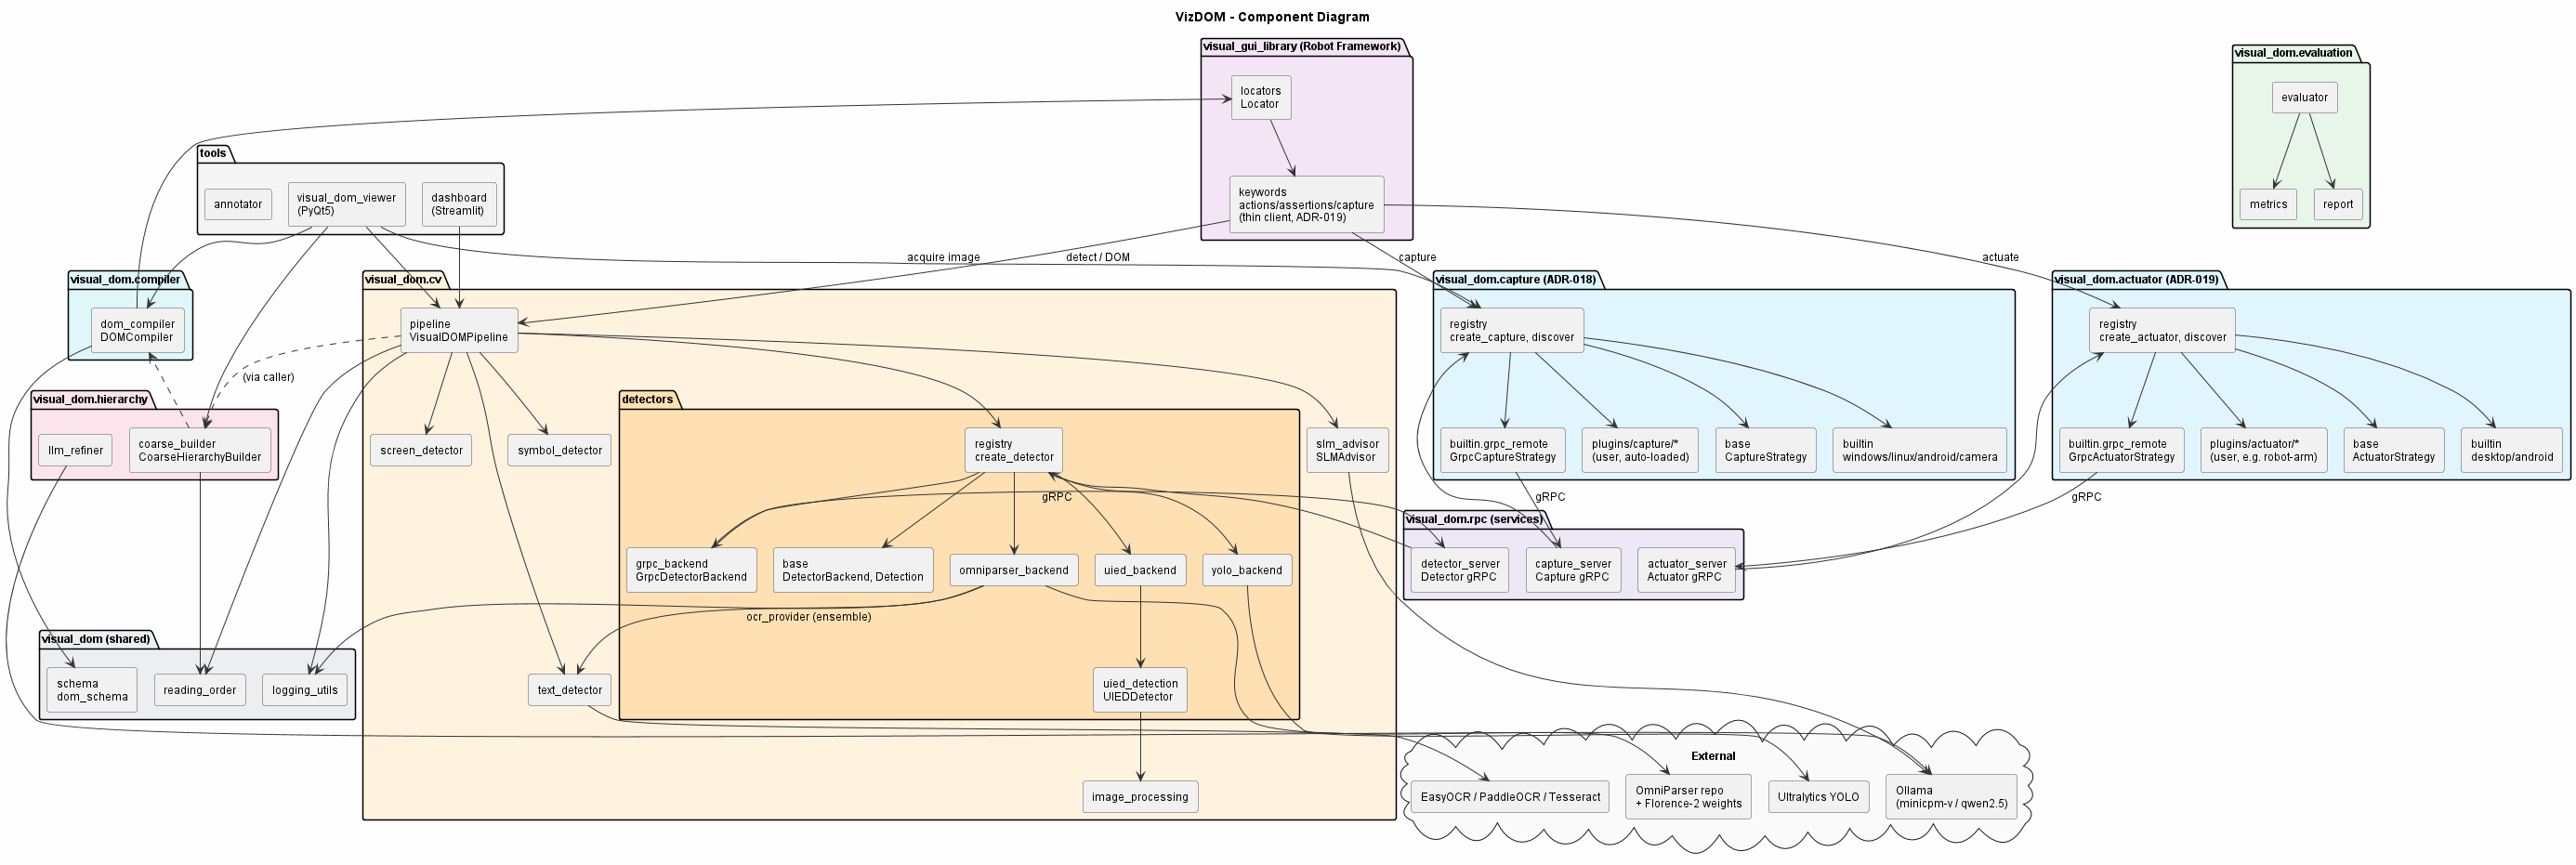
\includegraphics[width=\linewidth]{Component_Diagram.png}
  \caption{Khối xây dựng cấp 1/2 và phụ thuộc. Chú giải: hộp tô màu là gói; hộp lồng
  là gói con; mũi tên là ``phụ thuộc / gọi''. Ranh giới hệ thống: mọi thứ trừ đám mây
  \emph{External} (bộ OCR, trọng số OmniParser, Ollama, YOLO).}
  \label{fig:component}
\end{figure}

\section{Cấp 2 --- khuôn mẫu cổng bị điều khiển}
Mỗi cổng bị điều khiển (phát hiện, chụp, tác động) chia sẻ cùng cấu trúc nội bộ:
\begin{itemize}[leftmargin=1.4em]
  \item một \textbf{strategy cơ sở} (phương thức trừu tượng: ví dụ \code{detect} /
        \code{capture} / \code{tap+type+swipe});
  \item một \textbf{registry} phơi bày \code{create\_X(name)}, \code{list\_X()},
        \code{auto\_select()};
  \item \textbf{tự khám phá} nạp các built-in và bất kỳ plugin người dùng nào đặt
        trong một thư mục quy ước;
  \item một \textbf{strategy client gRPC} đăng ký dưới tên \code{grpc}, để một bộ
        điều hợp từ xa được chọn hệt như một bộ cục bộ.
\end{itemize}
Khuôn mẫu duy nhất này, lặp lại ba lần, là cơ chế đứng sau NFR1 và NFR2.

\section{Cấp 2 --- nội bộ pipeline thị giác}
Gói con \code{detectors} giữ giao diện \code{DetectorBackend}, một nhà máy registry,
và các backend UIED/YOLO/OmniParser/gRPC; pipeline còn sở hữu các bước
merge/split/NMS, hợp nhất thông minh, thứ tự đọc và rà soát SLM (Ch.~6).

% =====================================================================
\chapter{Góc nhìn Thời gian chạy}
% =====================================================================
\section{Kịch bản 1 --- ảnh sang DOM cục bộ (đường thuận lợi)}
Hình~\ref{fig:seq} minh họa một chu trình với bộ phát hiện OmniParser và bật rà soát
SLM. Luồng chi tiết của pipeline ở Hình~\ref{fig:pipeline}.

\begin{figure}[H]
  \centering
  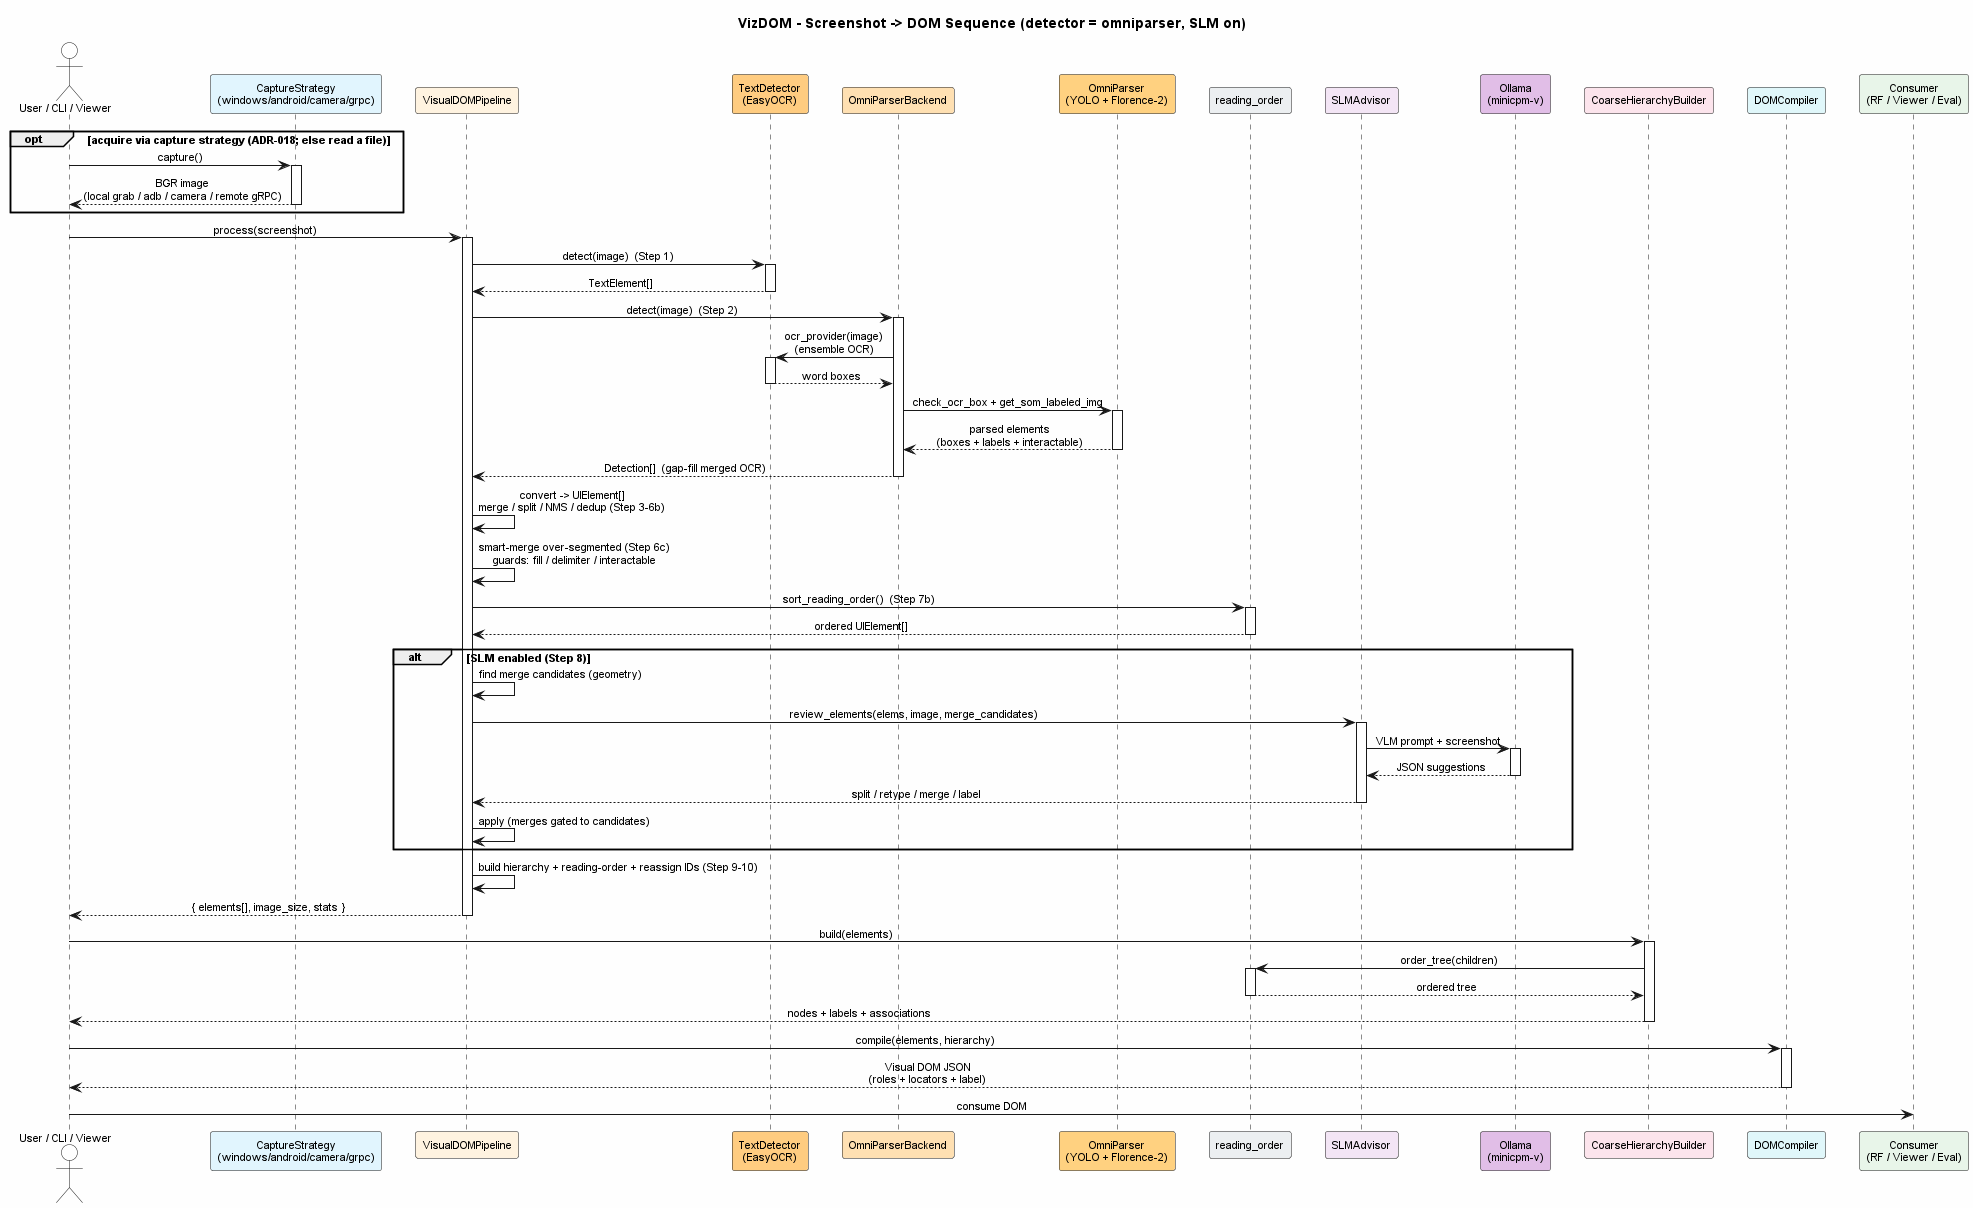
\includegraphics[width=\linewidth]{Sequence_Diagram.png}
  \caption{Kịch bản 1: chụp (tùy chọn) $\rightarrow$ OCR $\rightarrow$ phát hiện có
  tổng hợp OCR $\rightarrow$ làm sạch $\rightarrow$ thứ tự đọc $\rightarrow$ rà soát
  SLM tùy chọn $\rightarrow$ phân cấp $\rightarrow$ DOM.}
  \label{fig:seq}
\end{figure}

\begin{figure}[H]
  \centering
  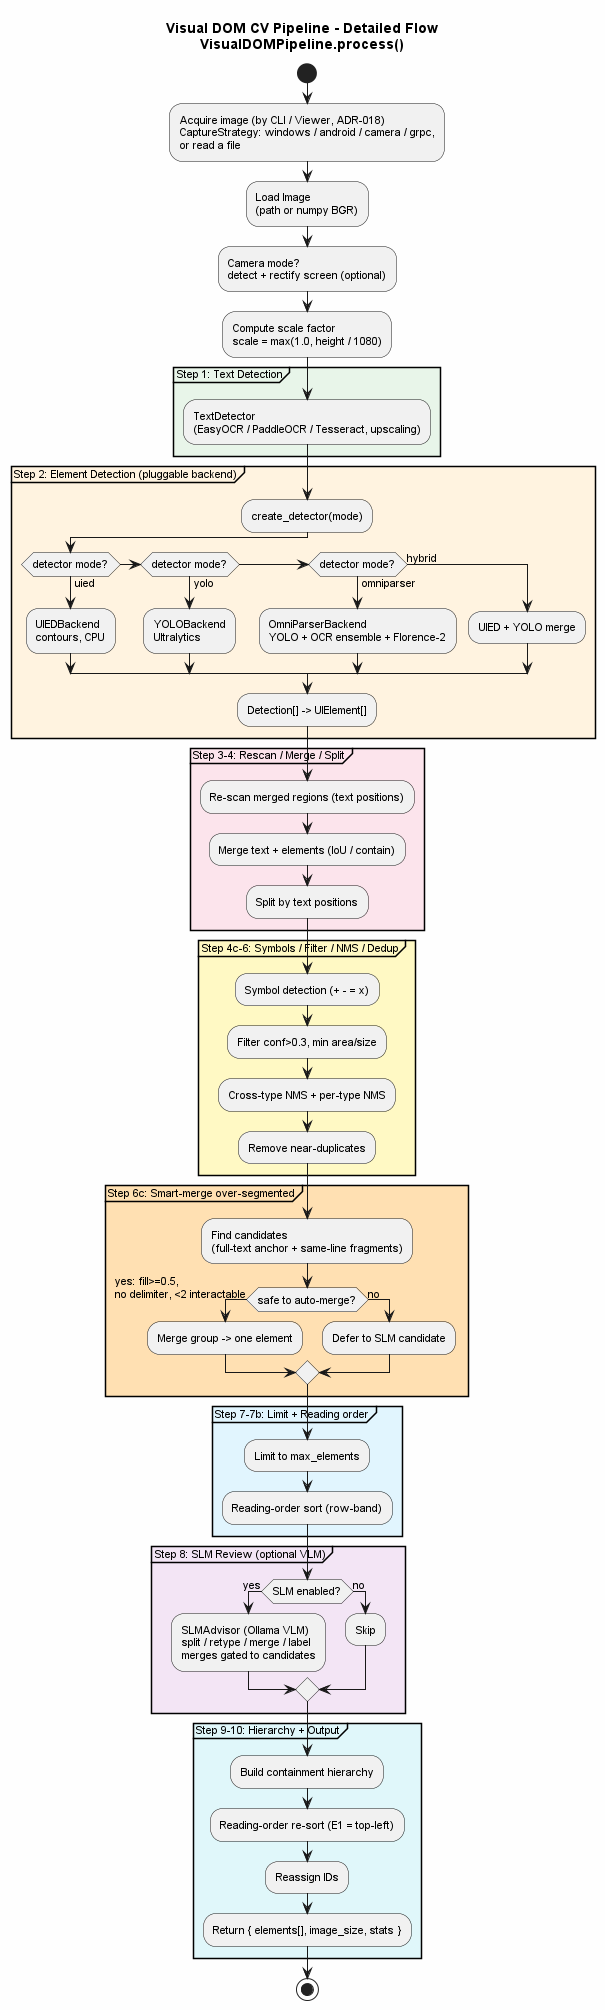
\includegraphics[height=0.82\textheight,width=\linewidth,keepaspectratio]{CV_Pipeline_Detail.png}
  \caption{Kịch bản 1, luồng điều khiển chi tiết của \code{VisualDOMPipeline.process()},
  gồm nhánh chọn bộ phát hiện và các quyết định hợp nhất thông minh / SLM có kiểm soát.}
  \label{fig:pipeline}
\end{figure}

\section{Kịch bản 2 --- chụp, phát hiện, tác động phân tán}
Một lần chạy kiểm thử được điều phối trên một client trong khi: chụp chạy trên thiết
bị cần kiểm thử (\code{grpc} chụp $\rightarrow$ dịch vụ chụp), phát hiện chạy trên máy
GPU (\code{grpc} phát hiện $\rightarrow$ dịch vụ phát hiện mô hình nóng), và tác động
chạy trên thiết bị hoặc bộ điều khiển cánh tay robot (\code{grpc} tác động
$\rightarrow$ dịch vụ tác động). Tọa độ chuẩn hóa đi trên đường truyền tác động và
được ánh xạ về không gian thiết bị ở phía máy chủ. Cấu trúc triển khai ở
Hình~\ref{fig:arch}.

\section{Kịch bản 3 --- các đường lỗi}
\begin{longtable}{@{}p{4.4cm}p{10.2cm}@{}}
\toprule
\textbf{Lỗi} & \textbf{Hành vi thiết kế} \\
\midrule
\endhead
Bộ phát hiện từ xa không tới được & Lời gọi client gRPC ném lỗi; CLI/trình xem hiển thị lỗi. Giảm nhẹ/dự phòng: chọn backend UIED tại chỗ (đổi cấu hình), không cần GPU hay mạng. \\
Ảnh xấu tới dịch vụ & Máy chủ kiểm tra và trả trạng thái \code{INVALID\_ARGUMENT}/\code{INTERNAL} kèm thông báo; tiến trình máy chủ vẫn sống (một yêu cầu xấu không bao giờ làm sập nó). \\
Bộ phát hiện phân mảnh quá mức & Hợp nhất thông minh dựa luật (bảo vệ tỉ lệ lấp đầy / ký tự phân tách / tương tác) và hợp nhất SLM có kiểm soát sửa phân mảnh; hợp nhất bị giới hạn vào ứng viên hình học nên các điều khiển khác nhau không bị gộp. \\
OCR bỏ sót văn bản & Tổng hợp OCR đưa OCR có phóng đại của ta vào OmniParser để phục hồi từ bị sót (khử trùng lặp lấp khoảng trống). \\
SLM/Ollama không sẵn có & Bước tinh chỉnh là tùy chọn; pipeline tiếp tục chỉ với kết quả CV. \\
\bottomrule
\end{longtable}

% =====================================================================
\chapter{Góc nhìn Triển khai}
% =====================================================================
\section{Phát triển / một máy}
Mọi cổng chạy tại chỗ trong một tiến trình Python; không dịch vụ nào được khởi động.
Đây là mặc định và là chế độ dùng để kiểm thử và chấm điểm.

\section{Phân tán}
\begin{figure}[H]
  \centering
  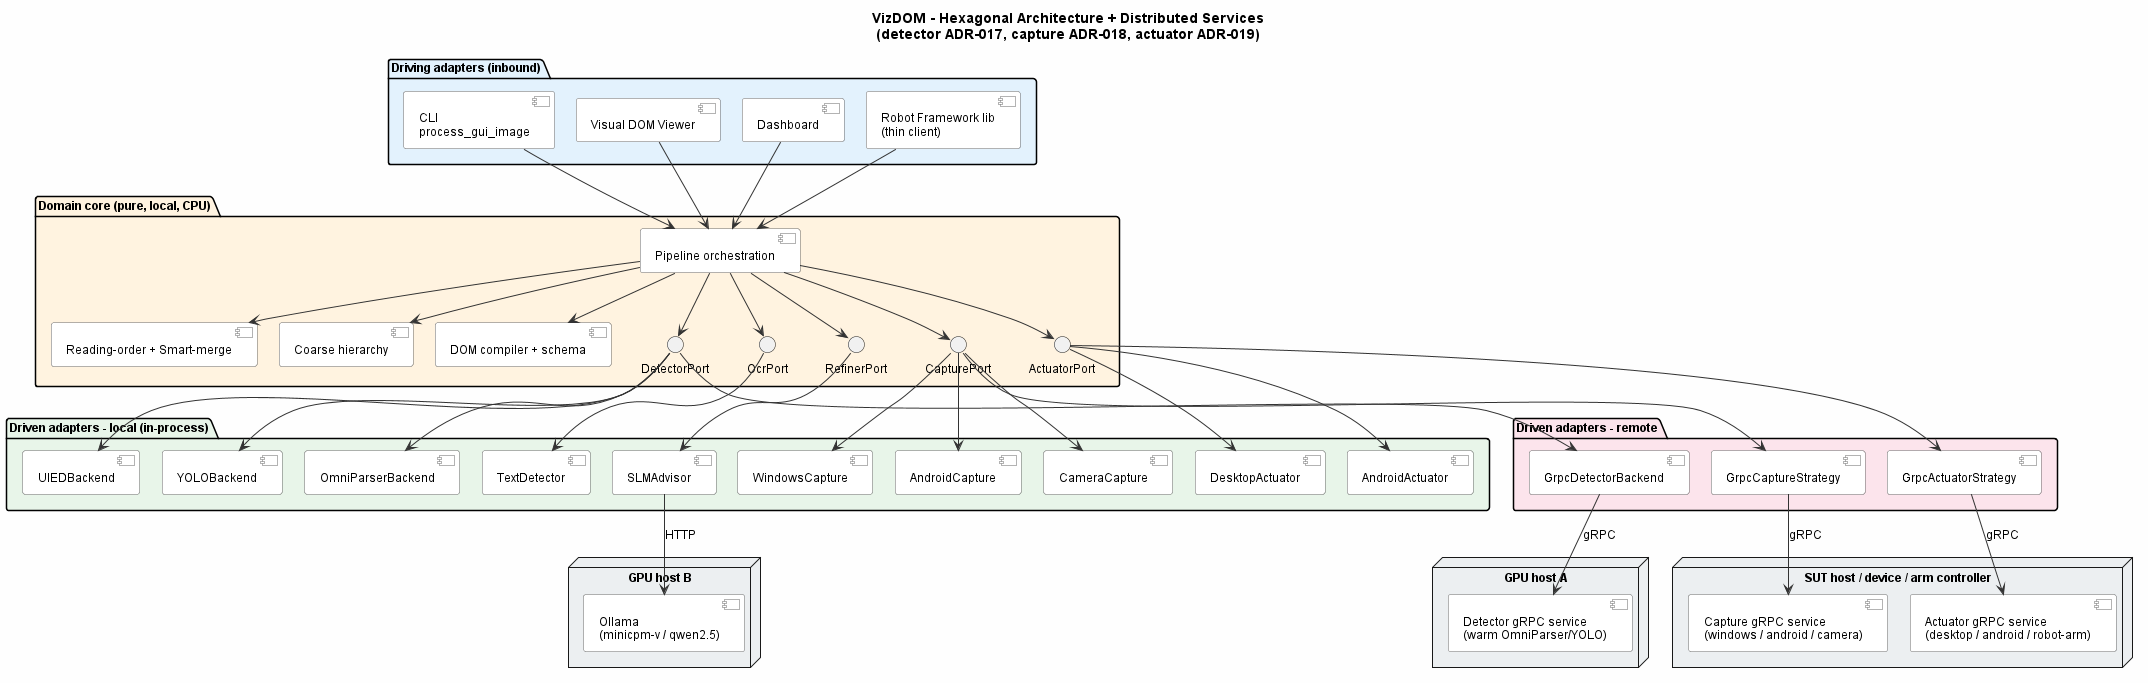
\includegraphics[width=\linewidth]{Architecture.png}
  \caption{Góc nhìn triển khai / cổng-và-bộ-điều-hợp. Bộ điều hợp điều khiển (trên)
  đi vào lõi; cổng bị điều khiển (dải giữa) gắn với bộ điều hợp cục bộ hoặc gRPC từ
  xa; dịch vụ gRPC chạy trên (các) máy GPU và bộ điều khiển SUT/cánh tay robot (dưới).
  Chú giải: hộp bo góc là thành phần; vòng tròn giao diện là cổng; hộp 3-D là nút
  triển khai; cạnh gán nhãn gRPC/HTTP là lời gọi mạng.}
  \label{fig:arch}
\end{figure}

\begin{longtable}{@{}p{4.2cm}p{4.2cm}p{6.0cm}@{}}
\toprule
\textbf{Nút} & \textbf{Chạy} & \textbf{Ghi chú} \\
\midrule
\endhead
Client / điều phối & CLI hoặc Robot Framework + lõi nghiệp vụ & Chọn chiến lược \code{grpc}; không giữ mô hình nặng. \\
Máy GPU & Dịch vụ gRPC phát hiện & OmniParser/YOLO nóng; \code{:50051}. \\
Máy/thiết bị SUT & Dịch vụ gRPC chụp + tác động & \code{:50053} / \code{:50054}; nơi ứng dụng cần kiểm thử chạy. \\
Bộ điều khiển cánh tay robot & Dịch vụ gRPC tác động (plugin cánh tay robot) & Áp dụng hiệu chỉnh ảnh$\rightarrow$vật lý. \\
Máy LM & Ollama & HTTP; tinh chỉnh tùy chọn. \\
\bottomrule
\end{longtable}

Khả quan sát: một logger tệp xoay vòng dùng chung (\code{logging\_utils}) với id
tương quan trên mỗi yêu cầu gRPC; thời gian mỗi yêu cầu được mỗi dịch vụ ghi log.

% =====================================================================
\chapter{Khái niệm Xuyên suốt}
% =====================================================================
\begin{description}[leftmargin=0pt,style=nextline]
  \item[Khả mở rộng (strategy + registry + tự khám phá)] Khái niệm quan trọng nhất;
    xem Ch.~5. Một plugin là một tệp kế thừa strategy cơ sở, tự nạp theo tên.
    \emph{Lưu ý an toàn:} khám phá nạp mã plugin --- chỉ dùng plugin tin cậy.
  \item[Hợp đồng tọa độ chuẩn hóa] Hành động tác động dùng tọa độ trong $[0,1]$ cộng
    kích thước ảnh nguồn; mỗi thiết bị ánh xạ về không gian của nó (desktop $\times$
    màn hình, android $\times$ độ phân giải đầu vào, cánh tay robot qua homography).
    Giữ bộ điều phối và giao thức độc lập với độ phân giải.
  \item[Dịch vụ mô hình nóng] Mô hình nặng nạp một lần mỗi tiến trình dịch vụ; client
    không trạng thái và rẻ.
  \item[Xử lý lỗi] Dịch vụ không bao giờ sập vì một yêu cầu xấu; trả trạng thái gRPC
    và tiếp tục phục vụ. Các bước tùy chọn (SLM, refiner) suy giảm êm.
  \item[Cấu hình] Chọn chiến lược theo tên từ cờ CLI / tham số thư viện / biến môi
    trường; đích cho cổng từ xa là chuỗi host:port.
  \item[Lưu trữ] Mỗi lần phân tích ghi vào thư mục phiên gắn dấu thời gian (ảnh, kết
    quả CV, DOM, siêu dữ liệu).
  \item[Giấy phép] Nghĩa vụ AGPL phát sinh khi backend OmniParser được phục vụ qua
    mạng; UIED là dự phòng không dính AGPL.
  \item[Hoạt động ngoại tuyến] Mã mô hình ngoài được đóng gói kèm và \emph{ghim} bằng
    script cài đặt; tài liệu kết xuất UML ngoại tuyến từ jar đóng gói kèm.
\end{description}

% =====================================================================
\chapter{Quyết định Kiến trúc}
% =====================================================================
Các quyết định được ghi dưới dạng ADR trong \code{docs/adr/}. Tập có ý nghĩa kiến
trúc (kèm trạng thái hiện tại) ở dưới; lưu ý ADR-017 vẫn \emph{Proposed} --- một điểm
lưu ý về kiểm chứng (Ch.~11).

\begin{longtable}{@{}p{1.4cm}p{7.8cm}p{2.4cm}@{}}
\toprule
\textbf{ADR} & \textbf{Quyết định} & \textbf{Trạng thái} \\
\midrule
\endhead
015 & Backend phát hiện cắm-thay được (UIED/YOLO/OmniParser) & Accepted \\
016 & Sắp xếp thứ tự đọc và nhãn phần tử & Accepted \\
017 & Kiến trúc lục giác phân tán với dịch vụ mô hình gRPC & \textbf{Proposed} \\
018 & Chụp màn hình cắm-thay được (strategy + dịch vụ) & Accepted \\
019 & Tác động đầu vào cắm-thay được (strategy + dịch vụ) & Accepted \\
\bottomrule
\end{longtable}

\section{ADR mẫu (rút gọn): ADR-019 Tác động đầu vào cắm-thay được}
\textbf{Bối cảnh.} Tác động đầu vào từng nằm trong các adapter Robot Framework, trùng
lặp với chụp và không có điểm cắm plugin (ví dụ một cánh tay robot). \textbf{Driver.}
NFR1 (khả sửa đổi), NFR2 (khả triển khai). \textbf{Quyết định.} Giới thiệu một
\code{ActuatorPort} --- bản sinh đôi phía-ghi của \code{CapturePort} --- với một
strategy cơ sở, một registry có tự khám phá, các built-in dời từ adapter RF, một hợp
đồng tọa độ chuẩn hóa và một dịch vụ gRPC tùy chọn. \textbf{Phương án.} (a) để đầu vào
trong RF (không có điểm cắm, chụp vẫn trùng lặp); (b) API tác động cấp-phần-tử (kéo
kiến thức DOM vào tầng thiết bị); (c) đường truyền tọa độ tuyệt đối (buộc bộ điều phối
biết độ phân giải mỗi thiết bị). \textbf{Hệ quả.} Loại bỏ trùng lặp; một thiết bị
cánh tay robot/card thu hình/serial là một plugin một-tệp; thư viện RF trở thành
client mỏng. Đánh đổi: hiệu chỉnh ảnh$\rightarrow$vật lý là việc thực sự, cô lập trong
plugin; tác động vật lý có nghĩa vụ an toàn mà plugin phải thực thi.

% =====================================================================
\chapter{Yêu cầu Chất lượng}
% =====================================================================
\section{Cây chất lượng (các chất lượng hàng đầu)}
Khả sửa đổi và Khả triển khai là gốc (xem xếp hạng driver), tiếp đến Khả kiểm thử,
rồi Độ chính xác và Hiệu năng.

\section{Kịch bản thuộc tính chất lượng}
\begin{longtable}{@{}p{2.2cm}p{12.4cm}@{}}
\toprule
\multicolumn{2}{@{}l}{\textbf{Q-01 --- Khả sửa đổi}} \\
\midrule
\endfirsthead
Driver & Thêm một backend phát hiện mới. \\
Kích thích & Một lập trình viên cần một bộ phát hiện mới (ví dụ một mô hình định vị khác). \\
Môi trường & Phát triển, lõi hiện có không đụng đến. \\
Tạo tác & Registry \code{visual\_dom.cv.detectors} + một tệp backend mới. \\
Phản ứng & Backend được khám phá và chọn được theo tên. \\
Đo phản ứng & 1 tệp mới + 1 dòng registry; \textbf{0} sửa lõi; cổng có $\geq 2$ hiện thực (hiện 4: UIED/YOLO/OmniParser/gRPC). \\
\bottomrule
\end{longtable}

\begin{longtable}{@{}p{2.2cm}p{12.4cm}@{}}
\toprule
\multicolumn{2}{@{}l}{\textbf{Q-02 --- Khả triển khai}} \\
\midrule
\endhead
Kích thích & Chuyển chụp về thiết bị và phát hiện về máy GPU. \\
Môi trường & Ba máy trên một mạng LAN. \\
Tạo tác & Cổng chụp/phát hiện + dịch vụ gRPC. \\
Phản ứng & Cùng một điều phối chạy, chọn chiến lược \code{grpc}. \\
Đo phản ứng & Chỉ đổi cấu hình (tên chiến lược + host:port); \textbf{0} đổi mã; vòng đầu-cuối thành công. \\
\bottomrule
\end{longtable}

\begin{longtable}{@{}p{2.2cm}p{12.4cm}@{}}
\toprule
\multicolumn{2}{@{}l}{\textbf{Q-03 --- Hiệu năng (mô hình nóng)}} \\
\midrule
\endhead
Kích thích & Một client gửi nhiều yêu cầu phát hiện liên tục. \\
Môi trường & Dịch vụ phát hiện trên một máy GPU. \\
Tạo tác & Dịch vụ gRPC phát hiện. \\
Phản ứng & Mô hình nạp một lần và tái dùng. \\
Đo phản ứng & Nạp mô hình đúng một lần mỗi vòng đời dịch vụ; các yêu cầu sau chỉ tốn suy luận. \\
\bottomrule
\end{longtable}

\begin{longtable}{@{}p{2.2cm}p{12.4cm}@{}}
\toprule
\multicolumn{2}{@{}l}{\textbf{Q-04 --- Khả kiểm thử}} \\
\midrule
\endhead
Kích thích & Chạy toàn pipeline và từ khóa RF trong CI trên một laptop. \\
Môi trường & Không GPU, không mạng. \\
Tạo tác & Lõi + UIED + chụp static-image + bộ tác động ghi lại. \\
Phản ứng & Sinh ra một DOM và từ khóa hành động mà không cần I/O thực. \\
Đo phản ứng & Lần chạy đầy đủ hoàn tất với không phụ thuộc GPU/mạng. \\
\bottomrule
\end{longtable}

\begin{longtable}{@{}p{2.2cm}p{12.4cm}@{}}
\toprule
\multicolumn{2}{@{}l}{\textbf{Q-05 --- Độ chính xác}} \\
\midrule
\endhead
Kích thích & Phát hiện phần tử trên các UI đại diện. \\
Môi trường & Tập điểm chuẩn gán nhãn. \\
Tạo tác & Bộ phát hiện + làm sạch + tinh chỉnh. \\
Phản ứng & Phát hiện khớp nhãn chuẩn. \\
Đo phản ứng & Mục tiêu F1 $\geq 0.80$, mIoU $\geq 0.60$. \emph{Đo được (tổng hợp, 44 ảnh, gộp):} F1 $0.51$ (UIED) / $0.58$ (OmniParser); chưa đạt mục tiêu F1, đạt mIoU (0.67--0.68). Recall điều khiển thao tác được (IoU$\geq$0.5): OmniParser nút 1.00, input 0.99, biểu tượng 0.67; UIED nút 0.82, input 0.95, hộp kiểm 0.68. Khả bấm trúng (center-hit): OmniParser 0.97, UIED 0.89. \\
\bottomrule
\end{longtable}

\section{Kế hoạch kiểm chứng}
\begin{longtable}{@{}p{2.0cm}p{5.4cm}p{4.4cm}p{2.2cm}@{}}
\toprule
\textbf{Kịch bản} & \textbf{Cách kiểm chứng} & \textbf{Chấp nhận} & \textbf{Trạng thái} \\
\midrule
\endhead
Q-01 & Đếm hiện thực mỗi cổng; thêm một backend trong test & $\geq 2$ hiện thực; 0 sửa lõi & \textbf{Đã kiểm chứng} (4 phát hiện, 5 chụp, 3 tác động) \\
Q-02 & Vòng gRPC đầu-cuối qua các tiến trình & chỉ cấu hình; vòng OK & \textbf{Đã kiểm chứng} về chức năng (chụp giống hệt từng điểm ảnh; tác động ánh xạ chính xác; phát hiện tái dùng nóng) \\
Q-03 & Đo số lần nạp mô hình trong dịch vụ & số lần nạp = 1 & \textbf{Đã kiểm chứng} về chức năng \\
Q-04 & Chạy pipeline + RF với bộ điều hợp CPU/static/ghi & hoàn tất, không I/O & \textbf{Đã kiểm chứng} \\
Q-05 & Chỉ số phát hiện trên tập tổng hợp (bộ khung) & F1 $\geq 0.80$, mIoU $\geq 0.60$ & \textbf{Đo được}: F1 0.58, mIoU 0.68; chưa đạt mục tiêu F1; OmniParser center-hit thao tác được 0.97 (R-04) \\
\bottomrule
\end{longtable}

% =====================================================================
\chapter{Rủi ro và Nợ Kỹ thuật}
% =====================================================================
\begin{longtable}{@{}p{1.2cm}p{5.0cm}p{2.0cm}p{5.6cm}@{}}
\toprule
\textbf{ID} & \textbf{Rủi ro / Nợ} & \textbf{Tác động / K.n.} & \textbf{Giảm nhẹ} \\
\midrule
\endhead
R-01 & ADR-017 (gRPC phân tán) đang \emph{Proposed}, nhưng bằng chứng NFR2 dựa vào nó & Cao / -- & Chấp nhận ADR-017 sau rà soát, hoặc hạ tuyên bố khả triển khai xuống ``đã minh chứng, chưa phê chuẩn''. \\
R-02 & Kênh gRPC chưa xác thực / chưa mã hóa & Cao / TB & Chỉ dùng LAN hiện tại; thêm TLS + xác thực (theo dõi tiếp). \\
R-03 & Tự khám phá plugin chạy mã người dùng; một bộ tác động có thể di chuyển cánh tay vật lý & Cao / Thấp & Chính sách plugin tin cậy; ghi nghĩa vụ an toàn (giới hạn, e-stop) là trách nhiệm plugin. \\
R-04 & F1 dựa IoU tổng thể dưới mục tiêu (0.58 vs 0.80); một chỉ số IoU đơn che giấu việc cả hai bộ phát hiện đều bấm-trúng-được cao & TB / Cao & Báo cáo center-hit cùng IoU; thêm tập gán nhãn thực tế; xem lại liệu mục tiêu F1 0.80 có phải mục tiêu vận hành đúng. \\
R-05 & Phân mảnh quá mức trên UI thực nhiều dải màu & TB / TB & Hợp nhất thông minh + SLM có kiểm soát; tiếp tục tinh chỉnh. \\
D-01 & Chỉ số chỉ phủ phát hiện phần tử + OCR (nhãn chuẩn thiếu cây / bộ định vị) & Thấp / -- & Trục phân cấp + bộ định vị chờ nhãn chuẩn dạng cây. \\
D-02 & Mã registry/khám phá trùng lặp trên 3 cổng & Thấp / -- & Tách một lớp registry-plugin dùng chung. \\
\bottomrule
\end{longtable}

\section{Phát hiện D-CAR (rà soát theo quyết định)}
\begin{longtable}{@{}p{4.6cm}p{5.0cm}p{4.4cm}@{}}
\toprule
\textbf{Quan sát} & \textbf{Ảnh hưởng} & \textbf{Hành động} \\
\midrule
\endhead
NFR2 truy về ADR-017, vốn \emph{Proposed} chứ không \emph{Accepted}. & Một tuyên bố driver hàng đầu dựa trên một quyết định chưa phê chuẩn. & Phê chuẩn ADR-017 hoặc phát biểu lại là chỉ-minh-chứng. (R-01) \\
Phân tán đã hiện thực nhưng quyết định an toàn là ngầm (kênh không bảo mật, chưa từng là ADR). & Quyết định ẩn; người rà soát không thấy được đánh đổi. & Viết một ADR cho an toàn truyền tải; thêm TLS. (R-02) \\
Khả sửa đổi được \emph{tuyên bố} và \emph{minh chứng} (4/5/3 hiện thực). & Tuyên bố mạnh, kiểm chứng được. & Giữ số đếm hiện thực được tái sinh từ repo. \\
F1 IoU$\geq$0.5 (0.58) dưới mục tiêu, nhưng center-hit cho thấy cả hai bộ phát hiện định vị tốt điều khiển thao tác được (OmniParser 0.97, UIED 0.89). & Một chỉ số IoU đơn đánh giá thấp tính hữu dụng vận hành. & Báo cáo center-hit + IoU; thêm tập thực tế; xem lại mục tiêu F1. (R-04) \\
\bottomrule
\end{longtable}

% =====================================================================
\chapter{Thuật ngữ}
% =====================================================================
\begin{longtable}{@{}p{3.8cm}p{10.8cm}@{}}
\toprule
\textbf{Thuật ngữ} & \textbf{Định nghĩa} \\
\midrule
\endhead
Visual DOM & Cây JSON tương tự UI Automator (khung bao, vai trò, văn bản, nhãn, bộ định vị, phân cấp) tổng hợp từ một ảnh chụp. \\
Port / Adapter & Ranh giới phụ thuộc trừu tượng (port) và hiện thực cụ thể của nó (adapter), theo kiến trúc lục giác. \\
Cổng bị điều khiển & Cổng mà lõi \emph{gọi} (Detector, Ocr, Refiner, Capture, Actuator). \\
Strategy & Một hiện thực hoán đổi được, chọn theo tên lúc chạy. \\
Registry & Nhà máy + cơ chế khám phá tìm và tạo các strategy. \\
Mô hình nóng & Mô hình giữ nạp trong một tiến trình dịch vụ tồn tại lâu để khấu hao chi phí nạp. \\
Tọa độ chuẩn hóa & Tọa độ trong $[0,1]$ của chiều rộng/cao ảnh, ánh xạ về không gian thiết bị bởi mỗi bộ tác động. \\
UIED & Bộ phát hiện phần tử CPU cổ điển, không phụ thuộc thư viện (đường cơ sở)~\cite{xie2020uied}. \\
OmniParser & Bộ phát hiện học máy: phát hiện biểu tượng YOLO + chú thích Florence-2 + OCR. \\
SLM / VLM & Mô hình ngôn ngữ / thị giác nhỏ dùng để rà soát phần tử tùy chọn. \\
Homography & Ánh xạ chiếu 3$\times$3 từ điểm ảnh sang tọa độ vật lý (hiệu chỉnh cánh tay robot). \\
\bottomrule
\end{longtable}

\bibliographystyle{plain}
\bibliography{references}

\end{document}
